\title{Entrevista}
\subtitle{com Michele Duarte de Menezes}
\maketitle
\begin{wrapfigure}{l}{0.15\textwidth}

\includegraphics[width=0.15\textwidth]{figuras/foto-michele.png}
\end{wrapfigure}
Nesta edição da \textit{Newsletter} da Comissão de Pedometria da Sociedade Brasileira de Ciência do Solo, entrevistamos a Professora Doutora Michele Duarte de Menezes para falar um pouco sobre a Pedometria, suas potencialidades, dificuldades e perspectivas futuras no Brasil. A Dra. Michele atualmente é professora da disciplina de  Mapeamento Digital de Solos e Pedologia Aplicada na Universidade Federal Rural do Rio de Janeiro (UFRRJ). Sua formação pós ensino médio foi realizada na Universidade Federal de Lavras (UFLA), contemplando graduação em Agronomia, mestrado e doutorado em Ciência do Solo na área de Gênese, Morfologia e Classificação dos Solos. Realizou parte do seu doutorado na Purdue University (Estados Unidos). Publicou recentemente um artigo discorrendo sobre a importância da integração entre o conhecimento de campo do pedólogo e uso de ferramentas  estatísticas na predição de classes e propriedades de solos para a produção mais rápida de mapas de solos com acurácia das informações \citep{MenezesEtAl:2013}.\\
\\
\textbf{Pedometria} - O que levou você a se interessar e estudar sobre o Mapeamento Digital de Solos (MDS) e em especial temas relacionados a pedometria?\\
\\
\textbf{Michele} - Tanto no mestrado (início em 2005) quanto no doutorado, minhas atividades envolveram levantamento de solos e suas interpretações. Já no início do mestrado, os sistemas de informação geográficas e os modelos digitais de elevação começaram a se tornar mais acessível. Aliado a isso, e com o intuito de tentar melhorar os mapas de solos, comecei a ler inicialmente sobre mapeamento digital. Lembro-me que o primeiro material que li em português, foi um documento da EMBRAPA intitulado Mapeamento Digital de Classes e Atributos de Solos - métodos, paradigmas e novas técnicas \citep{MendoncaSantosEtAl:2003}. Esse documento traz um resumo sobre diversas técnicas pedométricas. Comecei então a cursar disciplinas e testar tais técnicas durante o meu período de treinamento.\\
\\
\textbf{Pedometria} - Quais são os projetos de pesquisa que você está desenvolvendo na área de MDS?\\
\\
\textbf{Michele} - Os projetos que tenho participado envolvem mapeamento de solos e seus atributos. Sob o ponto de vista de técnicas, temos empregado principalmente técnicas geoestatísticas (krigagem ordinária e krigagem combinada com regressão) e lógica \emph{fuzzy} (Figura \ref{fig:tecnicas}) aliada ao conhecimento \emph{expert}. Além disso, as pesquisas envolvem também o desenvolvimento de funções de pedotransferência, o uso sistemas de informação geográfica e geomorfometria.\\
\\
\begin{figure}[htbp]
\centering
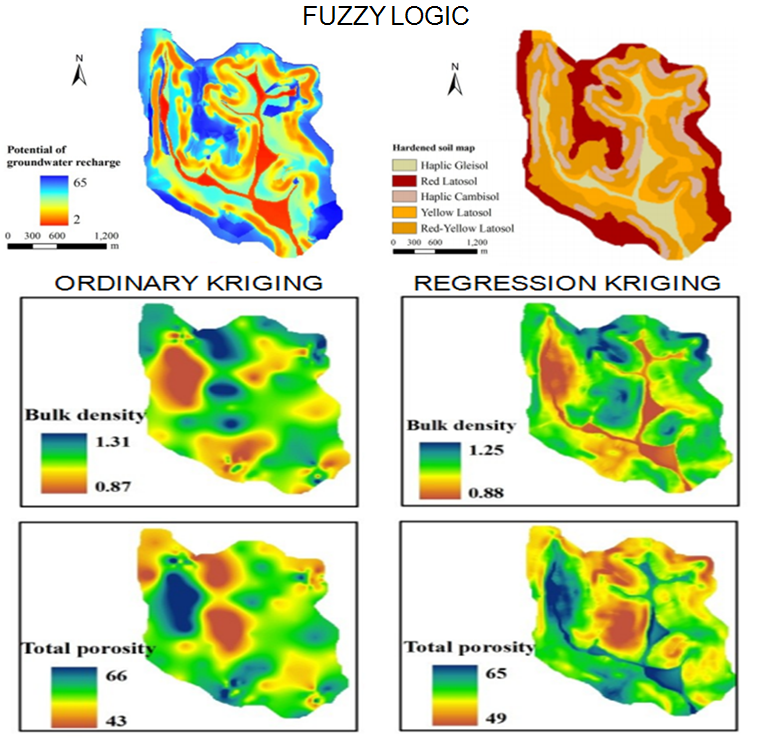
\includegraphics[scale=0.8]{figuras/tecnicas-predicao}
\caption{Técnicas de predição de atributos e classes de solos. Fonte: \cite{Menezes:2011}.}
\label{fig:tecnicas}
\end{figure}
\noindent \textbf{Pedometria} - O que você acha do cenário atual da pedometria no Brasil e qual o cenário que você vivenciou no seu doutorado sandwich em Purdue University nos EUA?\\
\\
\textbf{Michele} - Atualmente, tenho percebido um crescente interesse sobre a pedometria, por pessoas de diversas áreas do conhecimento da Ciência do Solo e outras áreas afins. No caso da UFRRJ, por exemplo, todas as disciplinas que envolvem técnicas pedométricas ou geotecnologias são muito procuradas na pós-graduação. Já nos Estados Unidos, o cenário foi um pouco diferente, pois eles já possuíam levantamento de solos em escalas mais detalhadas para grande parte do país, além de diversas interpretações a partir deles. A aquisição covariáveis ambientais para a predição é muito mais facilitada, como por exemplo, MDEs em elavada resolução gratuitamente disponíveis. Mais especificamente para o cenário de Purdue, as pesquisas estavam focadas principalmente na atualização dos mapas de solos já existentes, ou mesmo buscando gerar informações numéricas e continuamente distribuídas a partir do legado de solos (conhecimento tácito ou técnicas de mineração de dados).\\
\\
\textbf{Pedometria} - Qual a sua opinião a respeito da pedometria como uma disciplina nos cursos de Graduação e em especial nos Programas de Pós-Graduação na área de solos no Brasil?\\
\\
\textbf{Michele} - A pedometria tem um caráter multidisciplinar: eis um grande desafio para os cursos. A interação entre professores de diversas áreas do conhecimento é necessária. Além disso, vejo que existem muitos pré-requisitos acerca das técnicas de predição. Recentemente, foi ofertada aqui na UFRRJ uma disciplina chamada Métodos e Técnicas de Mapeamento Digital de Solos, ministrada pelos pesquisadores da EMBRAPA Solos Waldir de Carvalho Júnior, César da Silva Chagas, com minha colaboração. Diversas técnicas estatísticas e geostatísticas foram abordadas em aula, e um trabalho final usando uma base de dados real foi um dos requisitos. Percebi que os alunos tiveram dificuldade desde a formatação da base de dados, pois requeria um conjunto de operações em sistemas de informação geográfica, o que consiste em uma disciplina a parte. Outra dificuldade está relacionada à compreensão das técnicas em si (matemática, estatística e geostatística), o que exige muita leitura e compreensão mínima da linguagem 
matemática, onde teríamos talvez outra disciplina. Se formos pensar nas covariáveis ambientais, o uso do sensoriamento remoto é amplamente necessário, temos então mais uma nova disciplina complementar. Esses são apenas alguns exemplos que mostram que o desafio está em lidar efetivamente com esta multidisciplinaridade. Infelizmente, o processo de seleção dos programas de Pós-Graduação em Ciência do Solo estão cada vez mais específicos, dificultando o ingresso de alunos graduados em Matemática, Sistemas de Informação, Ciência da Computação, entre outros, o que seria salutar para o ensino e desenvolvimento da pedometria.\\
\\
\textbf{Pedometria} - Pela sua experiência na área de MDS, quais as principais dificuldades e desafios encontrados para os pesquisadores brasileiros desenvolverem seus trabalhos?\\
\\
\textbf{Michele} - Tanto para o pesquisador em MDS, quanto para outras áreas, as dificuldades são muito semelhantes, e geralmente de ordem burocrática. No entanto, de modo geral, os recursos disponíveis são crescentes para pesquisa. Pensando nas dificuldades do pesquisador em MDS, o foco no estabelecimento de infraestrutura é necessário, para um futuro impacto na qualidade dos produtos gerados. Nesse sentido, o desenvolvimento de um banco de dados de solos bem como a obtenção e livre disponibilização de informações ou mapas que representem covariáveis ambientais \ref{figure:covar}, em escalas mais detalhadas ou elevada resolução (exemplo: modelos digitais de elevação, mapas geológicos, uso e cobertura do solo, entre outros) são mais urgentes. Um dos desafios consiste na geração de novos dados de solos, como novas campanhas de campo, acompanhadas de técnicas de otimização amostral e o avanço do uso do sensoriamento remoto.\\
\\
\begin{figure}[htbp]
\centering
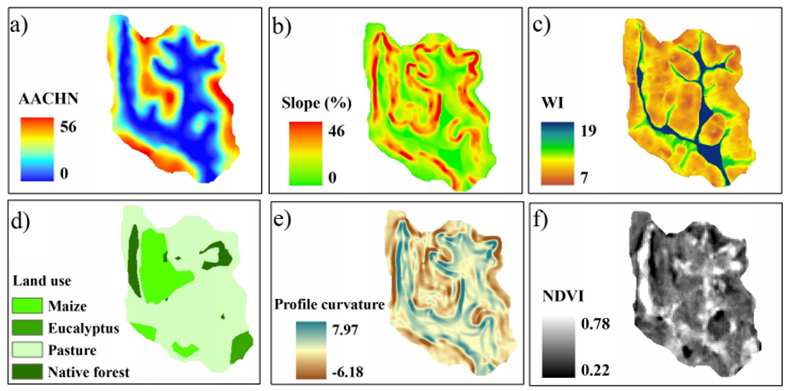
\includegraphics[scale=0.8]{figuras/covariaveis-ambientais}
\caption{Exemplos de covariávies ambientais utilizadas na predição de atributos do solo. Fonte: \cite{Menezes:2011}.}
\label{figure:covar}
\end{figure}
\noindent \textbf{Pedometria} - Você vê a pedometria como uma ferramenta promissora para ser utilizada na obtenção de informações de qualidade sobre solos e assim abastecer banco de dados de solos brasileiros?\\
\\
\textbf{Michele} - Sem dúvida a pedometria tem elevado potencial para geração de dados para um banco de dados. Acredito também no potencial dos pesquisadores brasileiros para implementar tais técnicas e gerenciar os dados. No entanto, o principal entrave não está no uso de técnicas, mas sim na burocracia acerca da política de dados no Brasil. Talvez por isso não tenhamos um banco de dados para todo território brasileiro até então.\\
\\
\textbf{Pedometria} - Qual a sua opinião a respeito da interdisciplinaridade nos grupos de pesquisa em MDS para desenvolver trabalhos de qualidade e que contribuam para meio científico? Na sua opinião, existe interdisciplinaridade nos grupos de pesquisa do Brasil? Sim ou Não? Por quê?\\
\\
\textbf{Michele} - A interdisciplinaridade atualmente é um desafio para várias áreas do conhecimento, e para o MDS não é diferente. Contudo, a interdisciplinaridade ou mesmo a integração entre diferentes órgãos, e não apenas de pesquisa, ainda é pouco efetiva no Brasil. Dentre vários motivos, a falta de efetividade é herdada da estrutura organizacional das universidades, além do fato de que professores não recebem treinamento para desenvolvimento de trabalhos interdisciplinares. Conheço alguns poucos projetos de pesquisa que buscam integração com diferentes áreas. Esta parceria deveria envolver as Universidades, IBGE, INPE, CPRM, EMBRAPA entre outros órgãos.\\
\\
\textbf{Pedometria} - Qual a sua opinião a respeito da abordagem e discussão da pedometria e do MDS no último Congresso Brasileiro de Ciência do Solo? Esses temas estão ganhando mais espaço nos eventos científicos de solos? Qual a situação do interesse do público leitor por temas relacionados a pedometria?\\
\\
\begin{figure}[htbp]
\centering
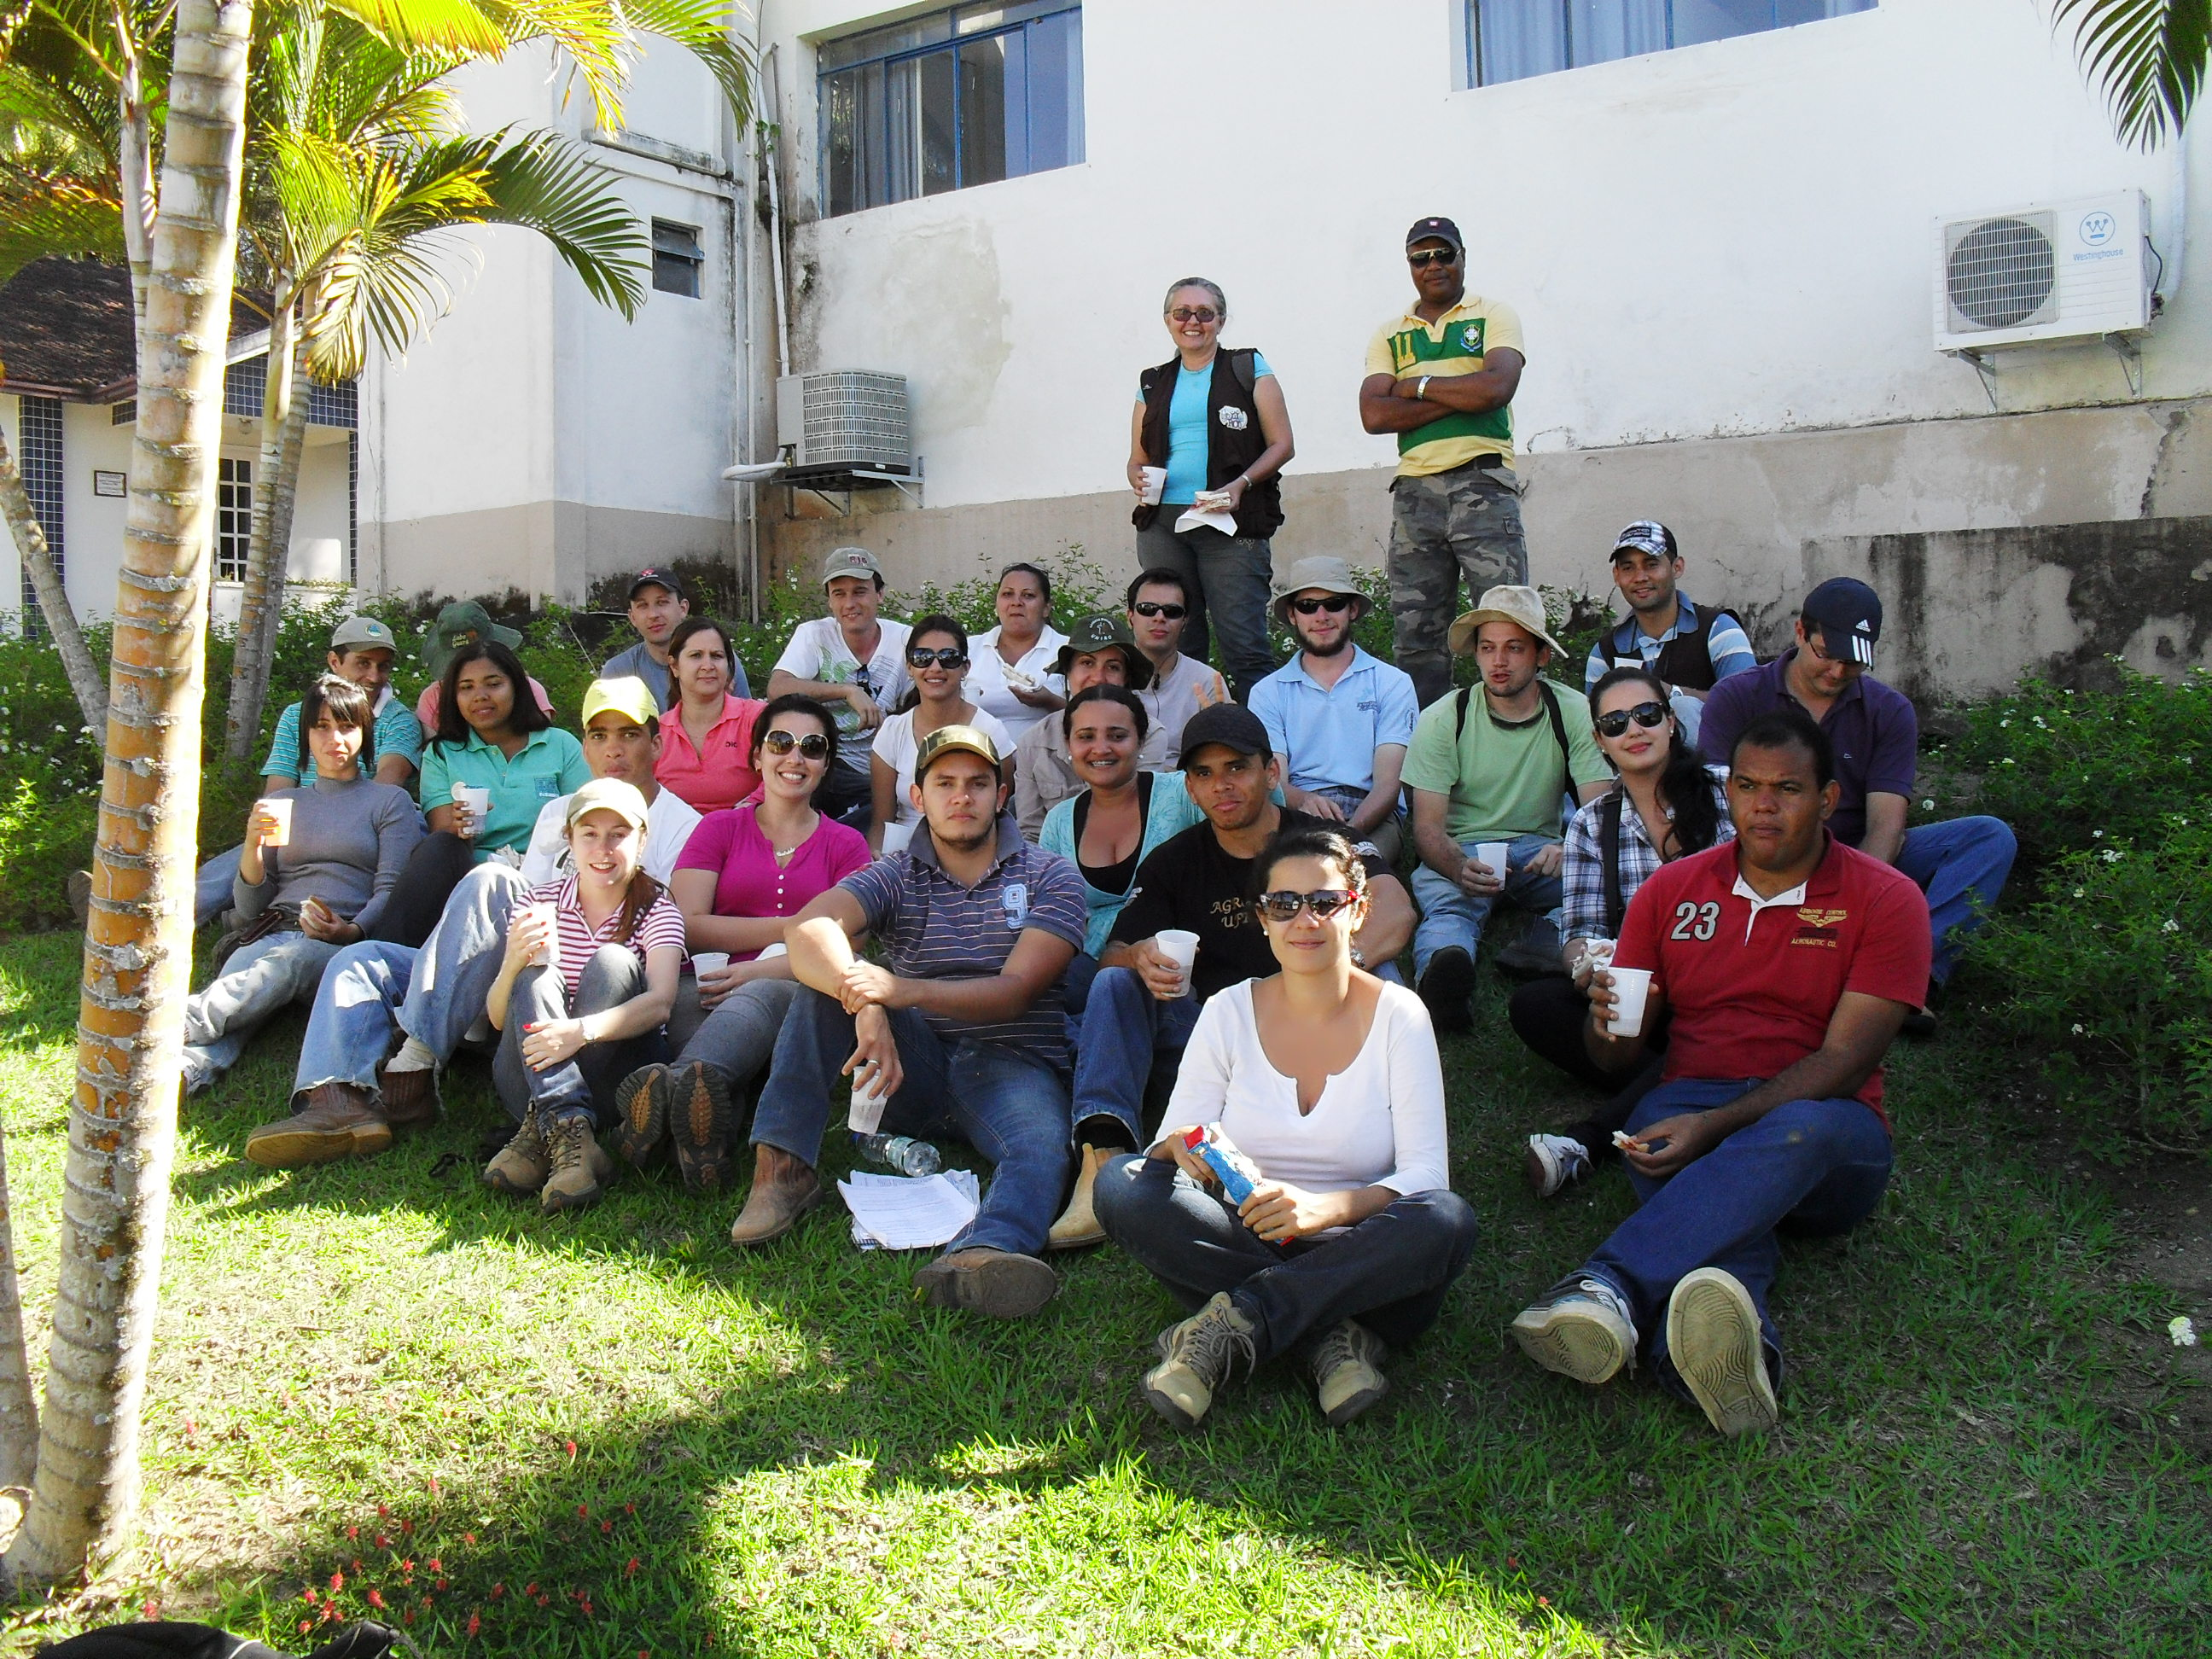
\includegraphics[scale=0.8]{figuras/michele-viagem}
\caption{A Dra. Michele (primeiro plano) acompanhando a prova de campo da disciplina de Formação e Caracterização do Solo da UFRRJ.}
\label{figure:covar}
\end{figure}
\noindent \textbf{Michele} - Creio que um dos assuntos mais comentados durante o Congresso desde ano foi a respeito da pedometria e o MDS, o que mostra um ganho de espaço nos eventos científicos ou mesmo enquanto linhas de pesquisa. Algumas palestras foram muito elucidativas, e espero que tenham acabado com alguns mitos ainda recorrentes acerca do MDS. Sim, os trabalhos de campo são de extrema importância ao mapeamento digital de solos. Não há dúvidas de que o conhecimento da Pedologia, Geomorfologia, Geologia, entre outras áreas, são fundamentais para o MDS e pedometria. Não, a pedometria não tem intuito de substituir a Pedologia, são áreas complementares ou afins. O próprio termo pedometria está relacionado à Pedologia (pedo), e metria está relacionada à parte da mensuração, a partir de métodos mais quantitativos (matemáticos e estatísticos).\\
A respeito do público leitor, creio que o interesse a respeito da pedometria tem crescido, principalmente entre pesquisadores e alunos de pós-graduação. Ao público em geral de outras áreas, acredito que soluções ambientais ou aplicações mais técnicas são mais interessantes.
\begin{footnotesize}
\begin{thebibliography}{99}
\bibitem[Mendonça-Santos \& Santos (2003) Mendonça-Santos \& Santos]{MendoncaSantosEtAl:2003}
M.L. Mendonça-Santos, H.G. Santos (2003)
\newblock Mapeamento digital de classes e atributos de solos: métodos, paradigmas e novas técnicas.
\newblock {\em Documentos} 55, 19p.
\bibitem[Menezes et~al. (2013) Menezes, Silva, Owens, Curi]{MenezesEtAl:2013}
M. D. Menezes, S. H. G. Silva, P. R. Owens, N. Curi (2013)
\newblock Digital soil mapping approach based on fuzzy logic and field expert knowledge.
\newblock {\em Ciência e Agrotecnologia} 37: 287-298. [\url{http://dx.doi.org/10.1590/S1413-70542013000400001}]
\bibitem[Menezes (2011) Menezes]{Menezes:2011}
M. D. Menezes (2011)
\newblock Levantamento pedológico de hortos florestais e mapeamento digital de atributos físicos do solo para estudos hidrológicos.
\newblock {\em Tese de doutorado, Universidade Federal da Lavras}, 225p.
\end{thebibliography} 
\end{footnotesize}
\address{Jean Michel Moura-Bueno\\
  Universidade Federal de Santa Maria\\
  \email{bueno.jean1@gmail.com}}
